\documentclass[a4paper,11pt]{article}

\usepackage[T1]{fontenc}
\usepackage[polish]{babel}
\usepackage[utf8]{inputenc}
\usepackage{lmodern}
\selectlanguage{polish}
\usepackage[top=2cm, bottom=2cm, left=3cm, right=3cm]{geometry}
\makeatletter
\newcommand{\linia}{\rule{\linewidth}{0.4mm}}
\renewcommand{\maketitle}{\begin{titlepage}
    \vspace*{2cm}
    \begin{center}\LARGE
    Politechnika Warszawska\\
    Wydział Elektryczny\\
    \end{center}
    \vspace{5cm}
    \noindent\linia
    \begin{center}
      \LARGE \textsc{\@title}
         \end{center}
     \linia
    \vspace{0.5cm}
    \begin{flushright}
    \begin{minipage}{5cm}
    \textit{Autorzy:}\\
    \normalsize \textsc{\@author} \par
    \end{minipage}
    \vspace{5cm}
     \end{flushright}
    \vspace*{\stretch{6}}
    \begin{center}
    \@date
    \end{center}
  \end{titlepage}%
}
\makeatother
\author{Grzegorz Kopyt\\
Daniel Sporysz}
\title{Specyfikacja Funkcjonalna \\
,,Automat Komórkowy - WireWorld''}
\usepackage{graphicx}

\begin{document}

\maketitle

\tableofcontents
\vspace{1cm}
\noindent\linia
\section{Opis działania}
Program jest implementacją automatu komórkowego opartego na regułach ,,gry w życie'' Johna Conwaya w wariancie ,,WireWorld''.

Za pomocą interfejsu graficznego program przedstawia zmiany pól jakie zachodzą na planszy zgodnie z zasadami gry.

Pracę programu można konfigurować na kilka sposobów: wczytać początkową konfigurację planszy z pliku graficznego, stworzyć własną planszę za pomocą narzędzi do edycji pól lub w sposób mieszany, czyli wczytując konfigurację z pliku i dalsza jego edycja za pomocą edytora programu.
Konfiguracji podlegają również metoda analizy planszy, jak również szybkość wyświetlania kolejnych przejść.

Analizę i modyfikację planszy można przerwać lub wznowić w każdej chwili pracy programu. Gdy generacja jest wstrzymana, użytkownik może ręcznie zmodyfikować planszę, zmienić sposób analizy planszy lub zapisać jej obecny stan do pliku graficznego.

Program umożliwia również ciągły zapis plansz do plików graficznych z których później możliwe jest stworzenie jednego pliku w formacie ,,GIF''.

\noindent\linia
\section{Funkcje}
Program oferuje następujące funkcje:
\begin{itemize}
\item Łatwa konfiguracja i obsługa pracy programu przez interfejs graficzny
\item Sterowane programem w czasie rzeczywistym - pauzowanie, wznawianie i ustawianie szybkości generowania kolejnych plansz
\item Odczyt planszy z pliku graficznego
\item Narzędzia do edycji planszy
\begin{itemize}
\item narzędzie ołówka, rysowania linii, gumka
\item wybór koloru
\end{itemize}
\item Określenie wymiarów planszy
\item Opcja wstawiania gotowych elementów z przygotowanej biblioteki obiektów WireWorld
\item Zapis aktualnego stanu planszy do pliku graficznego
\item Zapis ciągły generowanych pól do plików graficznych
\item Tworzenie plików .GIF
\item Czyszczenie planszy

\end{itemize}

\noindent\linia
\section{Obsługa}
Obsługa i konfiguracja pracy programu zachodzi przez interfejs graficzny.


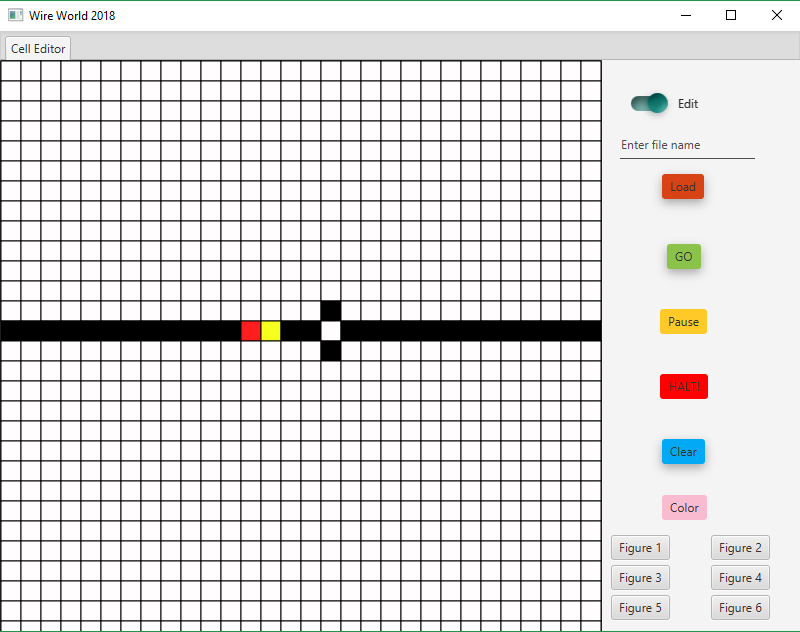
\includegraphics[width=\textwidth]{GUI_WireWorld}

\begin{itemize}
\item Pasek ,,Edit''  służy do włączania i wyłączania trybu edycji
\item Tryb edycji pozwala na edytowanie planszy poprzez klikanie na komórki lub przesuwanie po nich myszką z wciśniętym lewym przyciskiem myszy.
\item Komórki zmieniają kolory w kolejności ,,pusta''->,,przewodnik''->,,ogon''->,,głowa''->,,pusta''
\item W polu powyżej przycisku ,,Load'' należy podać ścieżkę pliku .png (1 piksel = 1 komórka), a następnie nacisnąć ,,Load''
\item Przycisk ,,GO" służy do uruchamiania animacji.
\item Przycisk ,,Pause'' służy do wstrzymywania animacji.
\item Przycisk ,,HALT!'' służy do zatrzymania animacji i ustawieniu jej w początkowej konfiguracji.
\item Przycisk ,,Clear'' powoduje zmianę koloru wszystkich komórek na kolor ,,pusta'.'
\item Aby wprowadzić figurę do planszy animacji należy nacisnąć przycisk z jej nazwa a następnie wybrać kratkę na planszy, od której ma się ona zaczynać.
\item Przycisk ,,Color'' przenosi do menu w którym można wybrać kolory stanów komórek.

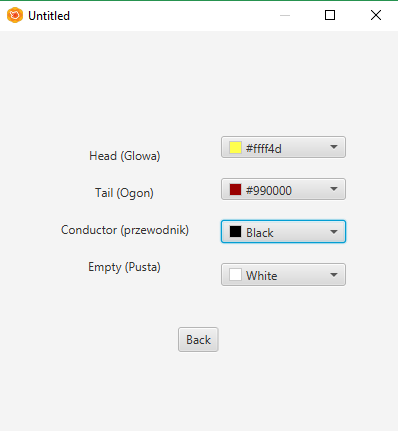
\includegraphics[width=\textwidth]{GUI_WireWorld_2}

\item Przy wybranej nazwie elementu należy wybrać kolor odpowiadającym przyciskiem z prawej kolumny.
\item Aby powrócić należy wcisnąć przycisk ,,Back''.

\end{itemize}

\noindent\linia
\section{Sytuacje wyjątkowe}
\begin{itemize}
\item Podano zbyt duże wymiary planszy
\item Plik graficzny zawiera planszę o zbyt dużych wymiarach
\item Podano złą ścieżkę do pliku graficznego
\item Podany plik nie jest plikiem graficznym
\item Program nie ma praw do odczytu plików 
\item Program nie ma praw do zapisu plików
\end{itemize}

\end{document}



